\documentclass[a4paper,10pt]{article}
\usepackage[utf8]{inputenc}
\usepackage[MeX]{polski}
\usepackage{graphicx}
\usepackage{hyperref}
\usepackage{fancyvrb}

\title{[WEDT.A] Klasyfikacja typów serwisów WWW na postawie informacji o~strukturze strony i~tekstu}
\author{Michał Aniserowicz, Jakub Turek}
\date{}

\begin{document}

\maketitle

\section*{Opis problemu}

Zadanie polega na implementacji aplikacji, która dokonuje automatycznej klasyfikacji typów stron WWW na podstawie ich  struktury. Analiza może obejmować źródło strony, konfigurację rozmieszczenia komponentów (layout), a~także strukturę i~znaczenie zamieszczonych na stronie treści.

\section*{Założenia}

Projekt obejmuje implementację klasyfikatora następujących typów serwisów:

\begin{description}
 \item [Blog] rodzaj internetowego dziennika (pamiętnika), który zawiera odrębnie, chronologicznie uporządkowane wpisy. Przykład serwisu: \url{http://rafalstec.blox.pl/}.
 \item [Serwisy informacyjne] portale zawierające najnowsze wiadomości z~różnych dziedzin życia, takich jak polityka, finanse, technologie. Przykład serwisu: \url{http://onet.pl/}.
 \item [,,Kwejki''] serwisy społecznościowe oparte w~głównej mierze na grafikach. Przykład serwisu: \url{http://kwejk.pl/}.
 \item [Sklepy internetowe] portale umożliwiające zakupy w~sieci przedmiotów z~różnych kategorii. Przykład serwisu: \url{http://allegro.pl/}.
\end{description}

Dane wejściowe aplikacji stanowić będzie adres witryny internetowej. Na wyjście wyprowadzona zostanie nazwa kategorii lub informacja, że serwis nie został zaklasyfikowany do żadnej z~powyższych kategorii.

\begin{figure}[h!]
\centering
  \begin{Verbatim}[frame=single,baselinestretch=0.3]
<div class="tooltip-title-container">

  <div class="tooltip-title-left-corner">

    <div class="tooltip-title">

      <p class="tooltip-title-h2">

        <a href="/obrazek/1763501/autor-gry-o-tron.html">

          Autor Gry o Tron?

        </a>

      </p>

    </div>

    <div class="tooltip-title-right-corner"></div>

    <div class="clr"></div>

  </div>

</div>
  \end{Verbatim}
  \caption{Fragment kodu źródłowego witryny http://kwejk.pl.}
  \label{fig:kwejk_listing}
\end{figure}


\section*{Struktura danych}

Aplikacja umożliwiać będzie budowanie pełnego drzewa HTML. W~korzeniu drzewa przechowywane będą następujące informacje:

\begin{itemize}
 \item Typ napotkanego taga HTML, na przykład \verb+<div>+, \verb+<h1>+.
 \item Dodatkowe atrybuty taga powiązane z~CSS - kaskadowymi arkuszami styli: identyfikator \verb+id="_"+, klasa \verb+class="_"+ oraz styl elementu \verb+style="_"+.
 \item Tekst zawarty pomiędzy tagiem otwierającym a zamykającym. Przykładowo dla kodu \verb+<a>Odnośnik</a>+ jest to fraza ,,Odnośnik''.
 \item Inne atrybuty kontekstowe związane z~poszczególnymi tagami:
 
    \begin{itemize}
      \item dla obrazka (\verb+<img>+) - jego rozmiar oraz źródło pochodzenia (lokalne - z domeny, którą analizujemy lub zewnętrzne - spoza niej),
      \item dla nagłówków (\verb+<h1>+, \verb+<h2>+, itd.) - rozmiar czcionki.
    \end{itemize}
\end{itemize}

\begin{figure}[h!]
\centering
  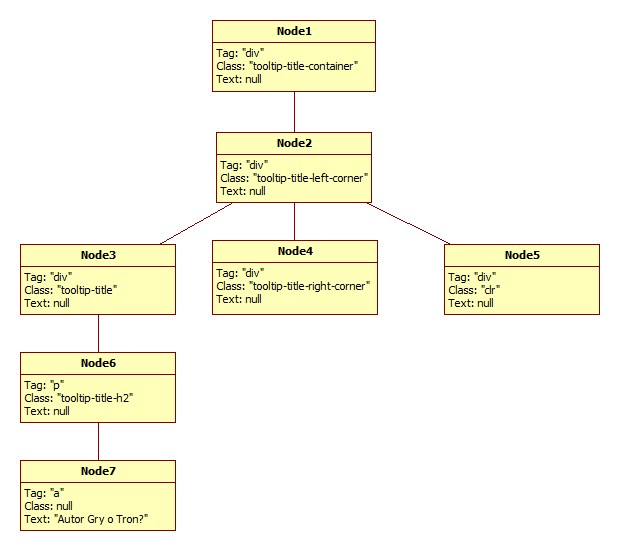
\includegraphics[width=\textwidth]{html_tree_full.jpg}
  \caption{Pełne drzewo HTML dla kodu przedstawionego na listingu \ref{fig:kwejk_listing}.}
  \label{fig:html_tree_full}
\end{figure}

Ze względu na rozmiary oraz skomplikowanie struktury dla dużych portali, takich jak sklepy internetowe lub serwisy informacyjne, kod aplikacji będzie udostępniał różne możliwości redukcji złożoności drzewa:

\begin{itemize}
 \item Zawężanie podzbioru tagów, dla których budowane jest drzewo. Tagi istotne dla struktury strony to, między innymi, \verb+<div>+, \verb+<td>+, \verb+<article>+, \verb+<h1>+, \verb+<a>+ oraz \verb+<img>+. Z~punktu widzenia zadania, tagi niosące niewiele informacji służą głównie do formatowania tekstu, jak na przykład \verb+<b>+, \verb+<span>+, oraz osadzania skryptów - \verb+<script>+.
 \item Ograniczanie stopnia zagnieżdżania korzeni w~drzewie:
    \begin{itemize}
	\item pomijanie węzłów przekraczających dany, parametryzowalny, poziom zagłębienia w~strukturze,
	\item sklejanie kilku następujących po sobie węzłów o~zbliżonych wymiarach na stronie w~jeden.
    \end{itemize}
 \item Odfiltrowywanie elementów uznanych za nieistotne metodami heurystycznymi, przykładowo prosty filtr eliminujący reklamy bazując na klasach obiektów.
\end{itemize}

\begin{figure}[h!]
\centering
  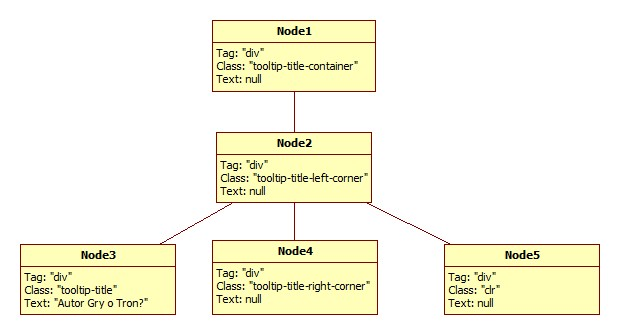
\includegraphics[width=\textwidth]{html_tree_cropped.jpg}
  \caption{Drzewo HTML z~rysunku \ref{fig:html_tree_full} zredukowane do tagów div.}
  \label{fig:html_tree_cropped}
\end{figure}

\end{document}